\section{Resultados}


Para criar o modelo do sistema solar tomaram-se algumas liberdades em relação
à distância dos planetas ao Sol, e como tal os valores das translações são mais
ou menos obtidos por experimentação. 

Os resultados obtidos estão nas imagens seguintes.






\begin{center}
 	
 	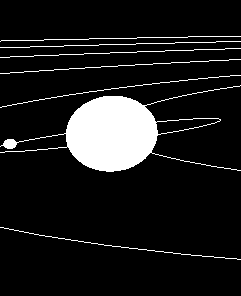
\includegraphics[width=0.5\textwidth,height=0.5\textheight,keepaspectratio]{resources/orbita_lua.png}
 	\captionsetup{type=figure, width=0.8\linewidth}
	\caption{\textit{Rendering} do modelo com foco na órbita da Lua}
\label{fig:ssec3:tilt} 
\end{center}


A \emph{Figura~\ref{fig:ssec3:modelo}} mostra o modelo com cometa. 

\begin{center}
 	
 	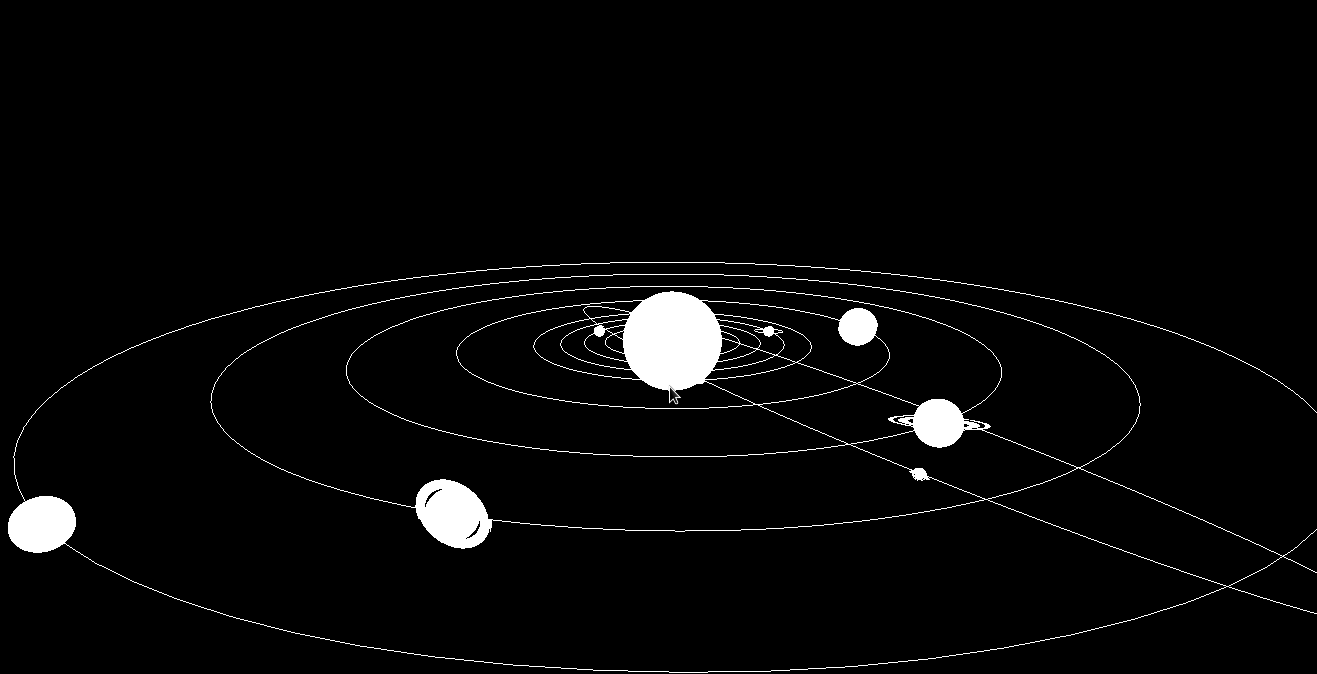
\includegraphics[width=\textwidth,height=\textheight,keepaspectratio]{resources/cometa.png}
 	\captionsetup{type=figure, width=0.8\linewidth}
	\caption{\textit{Rendering} do modelo final}
\label{fig:ssec3:modelo} 
\end{center}
